\documentclass{article}
\usepackage[margin=0.65in]{geometry}
\usepackage[utf8]{inputenc}

% Get better typography
\usepackage[protrusion=true,expansion=true]{microtype}	
% For algorithms
\usepackage[boxruled,linesnumbered,vlined,inoutnumbered]{algorithm2e}
\SetKwInOut{Parameter}{Parameters}
% For basic math, align, fonts, etc.
\usepackage{amsmath}
\usepackage{amsthm}
\usepackage{amssymb}
\usepackage{mathtools}
\usepackage{mathrsfs}
\usepackage{rotating}
\usepackage{soul}
\usepackage{gensymb} % For \degree
\usepackage{lscape}
% For \thead to make line breaks in tables
\usepackage{array}
\usepackage{makecell}
\renewcommand\theadalign{bc}
\renewcommand\theadfont{\bfseries}
\renewcommand\theadgape{\Gape[4pt]}
\renewcommand\cellgape{\Gape[4pt]}
\usepackage{courier} % For \texttt{foo} to put foo in Courier (for code / variables)
\usepackage{lipsum} % For dummy text
% For images
\usepackage{graphicx}
\usepackage{subcaption}
\usepackage[space]{grffile} % For spaces in image names
% For bibliography
\usepackage[round]{natbib}
% For color
\usepackage{xcolor}
\definecolor{light-grey}{rgb}{0.9,0.9,0.9}
\definecolor{dark-red}{rgb}{0.4,0.15,0.15}
\definecolor{dark-blue}{rgb}{0,0,0.7}
\usepackage{environ}
% Only show sections in table of contents and rename
\setcounter{tocdepth}{2}
\renewcommand{\contentsname}{Table of Contents}
% For links (e.g., clicking a reference takes you to the phy)
\usepackage{hyperref}
\hypersetup{
    colorlinks, linkcolor={dark-blue},
    citecolor={dark-blue}, urlcolor={dark-blue}
}

\newcommand{\TODO}[1]{\textcolor{blue}{\textbf{{#1}}}}
\newcommand{\WARNING}[1]{\textcolor{red}{\textbf{{#1}}}}
\newcommand{\POINTS}[1]{\textcolor{purple}{\textbf{{#1}}}}


\begin{document}


%-----------------
%	Homework 3
%-----------------
\newpage
\begin{center}
    \begin{Large}
    CMPSCI 687 Homework 3 - Fall 2022 
    \end{Large}
    \\
    Due \TODO{October 27, 2022}, 11:55pm Eastern Time
\end{center}
\addcontentsline{toc}{subsection}{\textbf{Homework 3}}

\vspace{0.25in}

\section{Instructions}

This homework assignment consists of a written portion and a programming portion. While you may discuss problems with your peers (e.g., to discuss high-level approaches), you must answer the questions on your own. In your submission, do explicitly list all students with whom you discussed this assignment. Submissions must be typed (handwritten and scanned submissions will not be accepted). You must use \LaTeX. The assignment should be submitted on Gradescope as a PDF with marked answers via the Gradescope interface. The source code should be submitted via the Gradescope programming assignment as a .zip file. Include with your source code instructions for how to run your code. You \textbf{must} use Python 3 for your homework code. You may not use any reinforcement learning or machine learning-specific libraries in your code, e.g., TensorFlow, PyTorch, or scikit-learn. You \textit{may} use libraries like numpy and matplotlib, though. The automated system will not accept assignments after 11:55pm on October 27. The tex file for this homework can be found \href{https://people.cs.umass.edu/~bsilva/courses/CMPSCI_687/Fall2022/HWs/HW3_Source.zip}{here}.

\begin{center}
    \WARNING{Before starting this homework, please review this course's policies on plagiarism by  \\reading Section 10 of the \href{https://people.cs.umass.edu/~bsilva/courses/CMPSCI_687/Fall2022/F22_687_Syllabus_v2.pdf}{\textcolor{red}{\underline{syllabus}}}.}
\end{center}

\noindent\rule{\textwidth}{1pt}

\section*{Part One: Written (50 Points Total)}
\begin{enumerate}

    \item (\POINTS{4 Points}) An operator $f$ is a contraction mapping if there exists some $\lambda \in [0,1)$ such that $d\big(f(x), f(y) \big) \leq \lambda d(x, y)$, where $d$ is a distance metric. Notice, here, that we explicitly forbid that $\lambda=1$, otherwise we would have no guarantees that the distance between $f(x)$ and $f(y)$ is smaller than the distance between $x$ and $y$. Assume, alternatively, that we try to ``fix'' this problem by defining $f$ to be a contraction mapping if there exists some $\lambda \in [0,1]$ such that $d\big(f(x), f(y) \big) < \lambda d(x, y)$. Notice that we now allow $\lambda=1$, but we require  $d\big(f(x), f(y) \big)$ to be strictly less than $\lambda d(x, y)$. What is the problem with this alternative definition of contraction mapping? What could go wrong if we were to use it?
    %
    % YOUR RESPONSE HERE
    %
    
    
    \vspace{0.8cm}
    \item (\POINTS{8 Points}) Let $M$ be an MDP with finite state space, finite action space, and $\gamma<1$. Let $\pi_1^*$ be an optimal policy that is \textit{stochastic}. Assume that we only know $\pi_1^*$, and that we \textit{do \underline{not} know} $v^{\pi_1^*}$ and $q^{\pi_1^*}$. Describe a procedure for transforming this (arbitrary) stochastic optimal policy, $\pi_1^*$, into a \textit{deterministic} policy, $\pi_2^*$, that is also optimal. Prove that the procedure you proposed guarantees that $\pi_2^*$ is indeed optimal. Hint: you can start from the definition of the Bellman Equation for $v^\pi$ (for an arbitrary policy $\pi$) and by recalling that $\sum_{x \in \mathcal X} \Pr(X=x) f(x) \leq \max f(x)$, where $X$ is a random variable with outcomes in $\mathcal X$ and $f$ is a function.
    %
    % YOUR RESPONSE HERE
    %
    
    
    \vspace{0.8cm}
    \item (\POINTS{5 Points}) In class, one of the definitions of optimal policy that we introduced is the following: $\pi^*$ is an optimal policy if and only if $\pi^* \geq \pi$, for all $\pi \in \Pi$. Here, the operator $\geq$ is defined so that $\pi \geq \pi'$ iff $v^\pi(s) \geq v^{\pi'}(s)$, for $\pi' \in \Pi$ and for all $s \in \mathcal{S}$. Suppose $\pi^*$ is the optimal policy for some MDP, e.g., Mountain Car. In Mountain Car, the initial state distribution, $d_0$, is defined such that the initial state of the car is $S_0=(X_0,0)$, where $X_0$ is the $x$ coordinate of the car at time $t=0$, drawn uniformly at random from the interval $[-0.6, -0.4]$. Suppose we \textit{change} the initial locations where the car may be initialized---i.e., suppose we change the initial state distribution, $d_0$, of Mountain Car. Consider, for instance, an alternative formulation of this MDP in which the car's initial $x$ coordinate, $X_0$, is drawn from a Gaussian distribution $\mathcal{N}(-0.3, 0.1)$. Without assuming anything about the new initial state distribution, is it possible to say that (in general) the optimal policy for the alternative formulation of Mountain Car is different than the optimal policy for the original problem? If so, prove that this is the case. If not, argue formally why the corresponding optimal policies may not differ.
    %
    % YOUR RESPONSE HERE
    %        
    
    
    \newpage
    \item (\POINTS{18 Points}) In class, we proved that the Bellman Operator is a contraction mapping and used this to show that Value Iteration converges to a unique fixed point. In the last homework, we investigated a function, $w^\pi(s, a, s')$, which represents the expected return if the agent starts in state $s$, executes action $a$, transitions to a particular next state $s'$, and then follows policy $\pi$. In this problem you will prove that a new form of dynamic programming Policy Evaluation operator, defined over $w^\pi$,  exists and is also a contraction mapping. This way, you will be showing that this Policy Evaluation procedure/operator can be used to compute $w^\pi$ (for any policy $\pi$) and that it converges to a unique fixed point.
    
    \begin{itemize} 
        \item In this question, the following identities/properties might be helpful:
        \vspace{0.2cm}\\
        \textbf{$\star$ Property 1}:
        \begin{equation}
        \label{eq:property1}
            \Big|\sum_{x \in \mathcal X} \Pr(X=x | Y=y, Z=z, \ldots) f(x, y, z, \ldots)\Big|\,\, \leq\,\, \sum_{x \in \mathcal X}\Pr(X=x | Y=y, Z=z, \ldots) \Big|f(x,y,z,\ldots)\Big|,
        \end{equation}
        where $X, Y, Z, \ldots$, are random variables with possible outcomes (respectively) in $\mathcal X, \mathcal Y, \mathcal Z, \ldots$,  and where $f$ is a function.
        \vspace{0.2cm}\\
        \textbf{$\star$ Property 2}:
        \begin{equation}
        \label{eq:property2}
            \sum_{x \in \mathcal X} \Pr(X=x | Y=y, Z=z, \ldots) f(x, y, z, \ldots)\,\, \leq\,\, \max_{x \in \mathcal X} f(x,y,z,\ldots),
        \end{equation}
        where $X, Y, Z, \ldots$, are random variables with possible outcomes (respectively) in $\mathcal X, \mathcal Y, \mathcal Z, \ldots$,  and where $f$ is a function.        
        \item Finally, let the Max-Norm over $w^\pi$ be defined as $||w^\pi||_\infty = \max_s \max_a \max_{s'} |w^\pi(s,a,s')|$.
    \end{itemize}
    
    \vspace{0.5cm}
    \textbf{(Question 4a.~\POINTS{4 Points})} In the last assignment, you showed how $v^\pi$ can be written/expressed in terms of $w^\pi$. Your expression for $v^\pi$ used only $w^\pi$, $\mathcal{S}, \mathcal{A}, p, R, d_0, \gamma$, and $\pi$. Based on this previous result, write a Bellman Equation for $w^\pi$ using only $w^\pi, \mathcal{S}, \mathcal{A}, p, R, d_0, \gamma$, and $\pi$ (but \ul{\textit{not}} $v^\pi$ or $q^\pi$). Your Bellman Equation for $w^\pi$ should resemble the form of the first Bellman Equation for $v^\pi$ we studied in class: $v^\pi(s) = \sum_a \pi(s,a) \sum_{s'} p(s,a,s') \, \big( R(s,a) \, + \, \gamma v^\pi(s') \big)$. In particular, your Bellman Equation for $w^\pi$  should have $w^\pi$ on both sides of the equation, but it should not depend on $q^\pi$ or $v^\pi$. Show your derivation of this new Bellman Equation step by step. 
    %
    % YOUR RESPONSE HERE
    %
    
    
    \vspace{0.75cm}    
    \textbf{(Question 4b.~\POINTS{14 Points})} Recall that we showed, in class, how the Bellman Optimality Equation for $v^*$,
    %
    $$v^*(s) = \max_a \sum_{s'} p(s,a,s') \, \big( R(s,a) \, + \, \gamma v^*(s') \big),$$
    %
    could be turned into an \textit{update equation}, used by the Value Iteration algorithm, to iteratively estimate $v^*$:
    %
    $$v_{i+1}(s) := \max_a \sum_{s'} p(s,a,s') \, \big( R(s,a) \, + \, \gamma v_{i}(s') \big).$$
    %
    To show that this update equation converges to $v^*$, we showed that the operator that implements it, $\mathcal T(v_i) := \max_a \sum_{s'} p(s,a,s') \, \big( R(s,a) \, + \, \gamma v_{i}(s') \big)$, is a contraction mapping. 
    % 
    Similarly, consider now the Bellman Equation for $w^\pi$ that you derived in the previous question. Turn it into an update equation that takes as input a current estimate, $w_i$, of $w^\pi$, and returns an updated estimate, $w_{i+1}$. Let $\Upsilon(w_i)$ be the operator that implements this update equation; that is, $\Upsilon(w_i)$ := $w_{i+1}$. Prove, step-by-step, that $\Upsilon$ is a contraction mapping under the $L^\infty$ norm (i.e., the same Max-Norm used in our proof that the Bellman Operator is a contraction). You may find it helpful to use the two properties described at the beginning of this question.
    %
    % YOUR RESPONSE HERE
    %

    
    \newpage
    \item (\POINTS{15 Points}) We showed in class that the Policy Iteration algorithm can---in the worst case--- converge to $\pi^*$ only in the limit, since the ``standard'' Policy Evaluation step may require an infinite number of iterations to converge. In this question, you will show that a \textit{different} way of performing the Policy Evaluation step can be used and allow for Policy Iteration to converge in a \textit{finite, bounded}, number of iterations. First, recall that in slides 55--58 of \href{https://umass.moonami.com/pluginfile.php/2297824/mod_resource/content/4/06_CS687.pdf#page=55}{Lecture 06}, we discussed how to perform policy evaluation by creating a system of linear equations with $|\mathcal S|$ equations and $|\mathcal S|$ unknowns. In particular, this system has one equation per state: the Bellman Equation for the corresponding state. As an example, consider an MDP with 2 states and 3 actions; the resulting system of equations would be:
    %
    \vspace{-0.05cm}
    %
    \begin{eqnarray*}
    v^\pi(s_1) &=& \sum_{a \in \{a_1, a_2, a_3\}} \pi(s_1,a) \sum_{s' \in \{s_1, s_2\}} p(s_1,a,s') \, \big( R(s_1,a) \, + \, \gamma v^\pi(s') \big) \\
    v^\pi(s_2) &=& \sum_{a \in \{a_1, a_2, a_3\}} \pi(s_2,a) \sum_{s' \in \{s_1, s_2\}} p(s_2,a,s') \, \big( R(s_2,a) \, + \, \gamma v^\pi(s') \big) \\
    v^\pi(s_3) &=& \sum_{a \in \{a_1, a_2, a_3\}} \pi(s_3,a) \sum_{s' \in \{s_1, s_2\}} p(s_3,a,s') \, \big( R(s_3,a) \, + \, \gamma v^\pi(s') \big).    
    \end{eqnarray*}
    
If $p$ and $R$ are known, one could expand each equation above and obtain formulas whose form resembles (for instance) something like $v^\pi(s_1) = 0.3 + 0.12 \gamma v^\pi(s_1) + 0.42 \gamma v^\pi(s_2) - 0.9 \gamma v^\pi(s_3)$. Consider the following MDP:

\begin{figure}[h!!!]
    \centering
    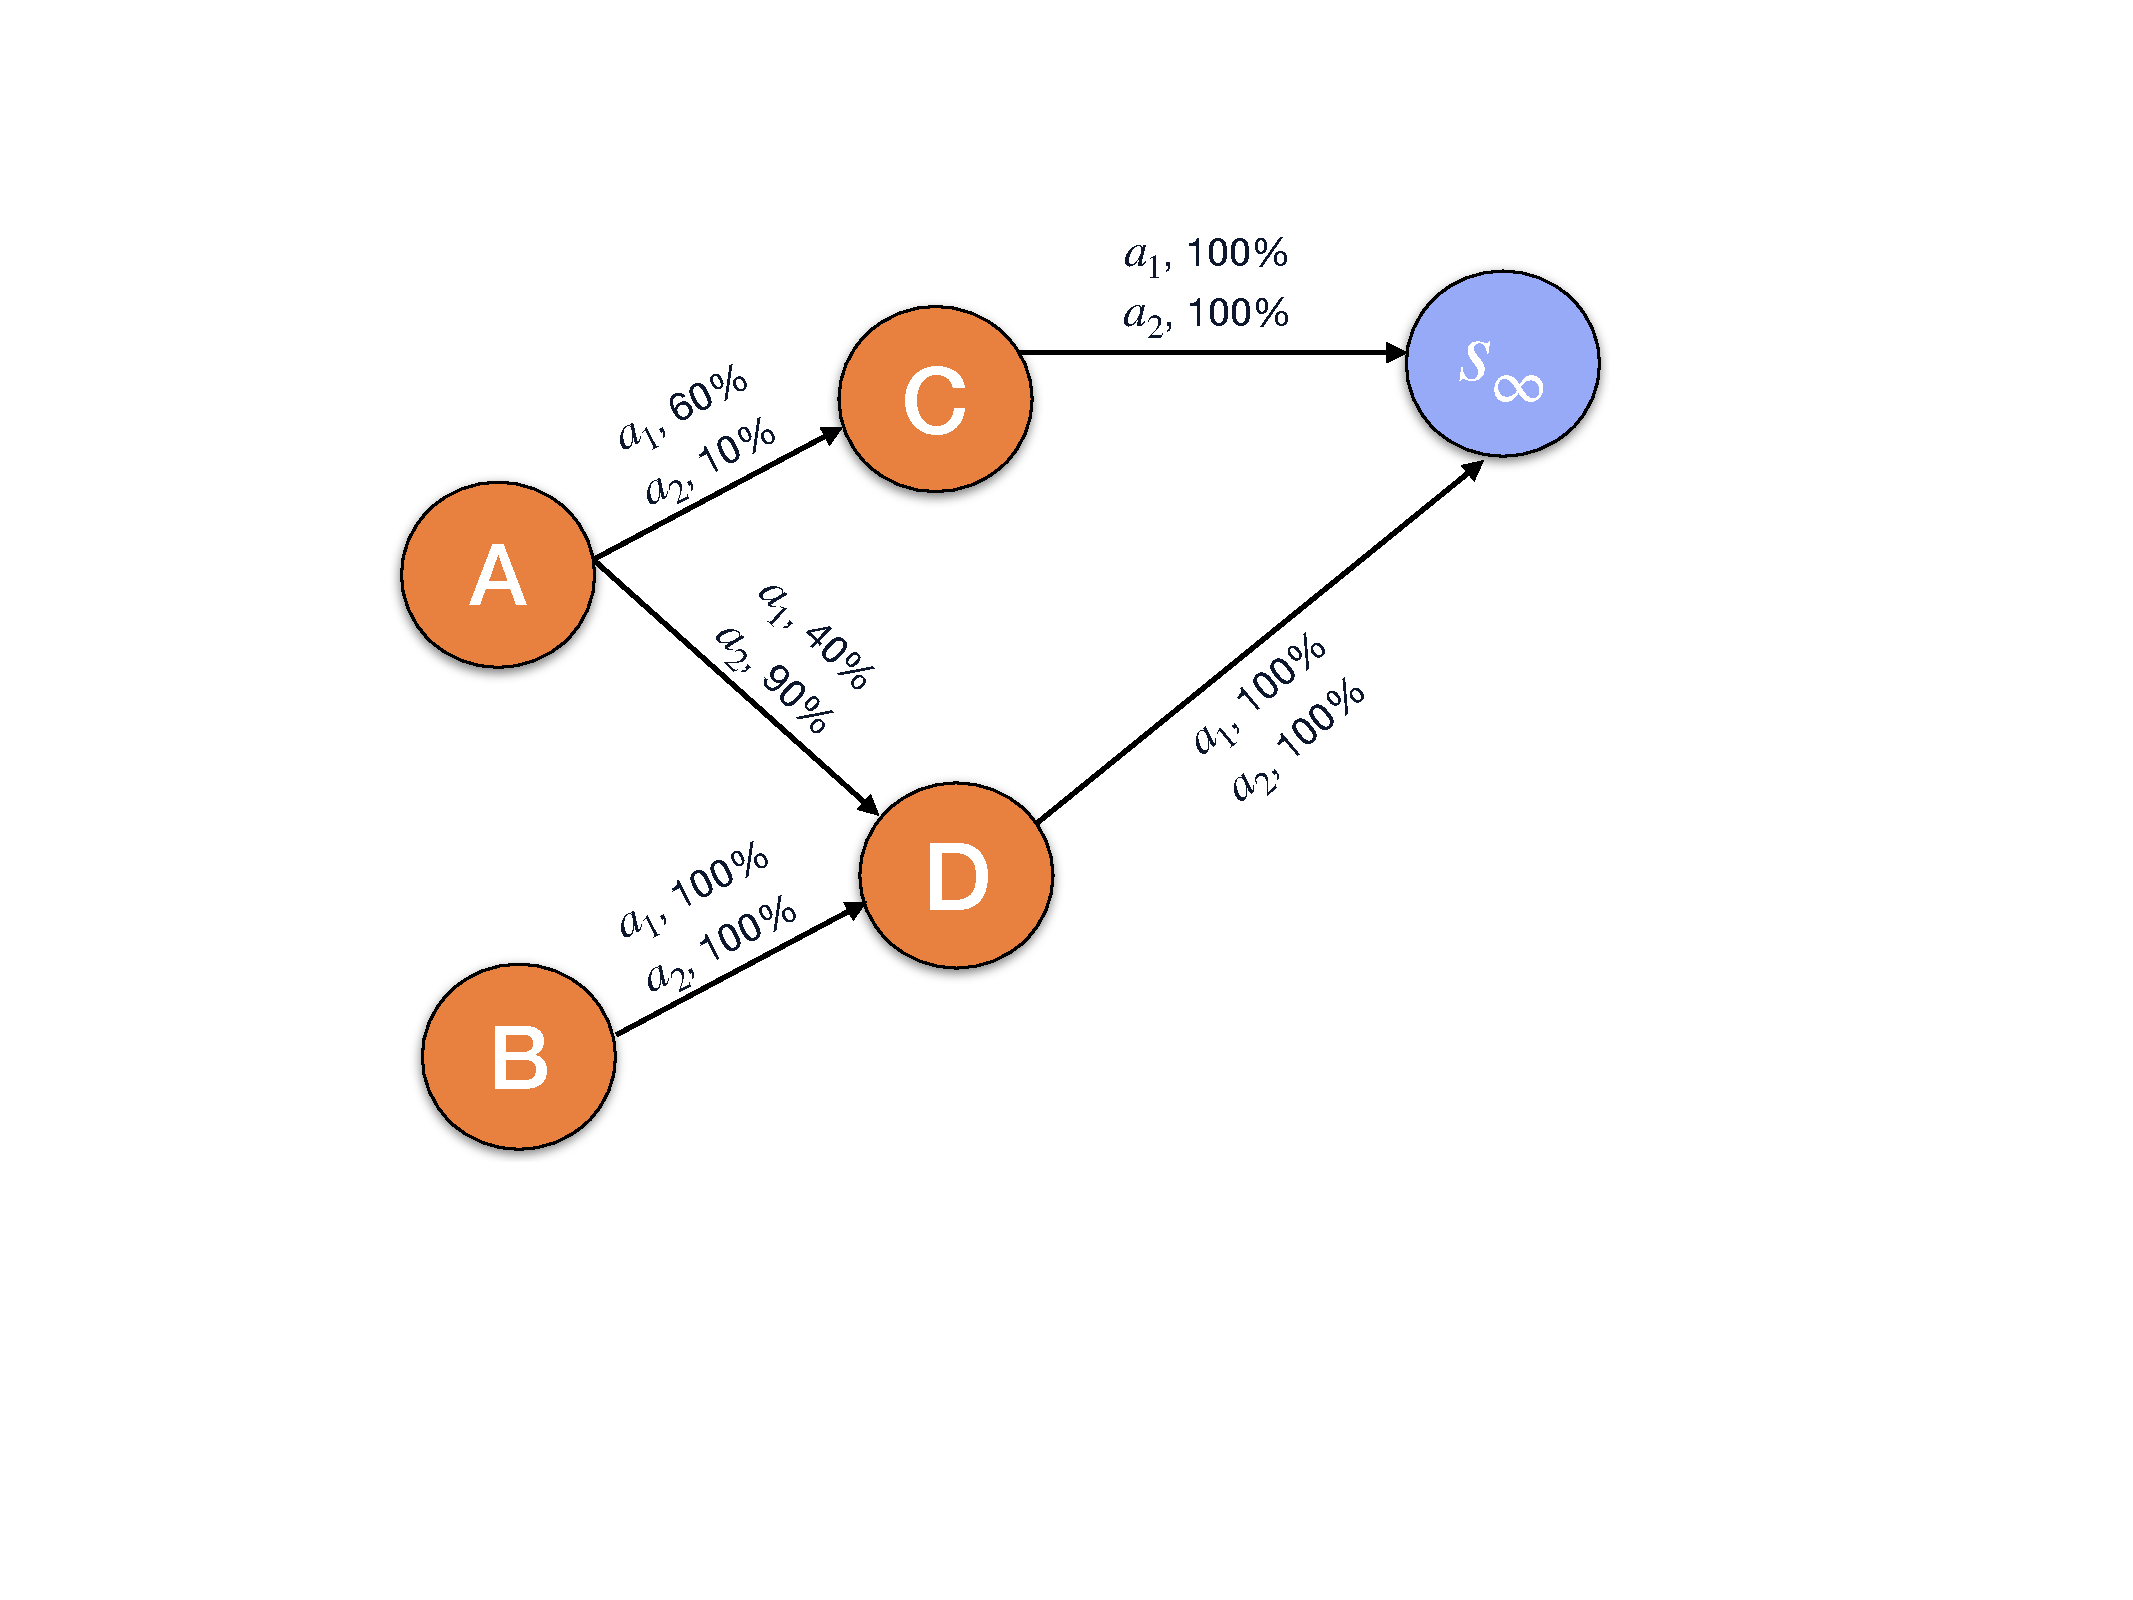
\includegraphics[width=0.32\textwidth]{HW_figs/HW3_MDP.pdf}
\end{figure}

Assume the following transition function, $p$, where all transition probabilities not indicated in the table below are $0$; the following reward function, $R$; and the following stochastic policy, $\pi$:

\begin{table}[h!!!!]
\centering
\footnotesize
\begin{tabular}[t]{|l|l|}
\hline
$p(A,a_1,C)=0.6$    &   $p(A,a_1,D)=0.4$ \\ \hline
$p(A,a_2,C)=0.1$    &   $p(A,a_2,D)=0.9$ \\ \hline
$p(B,a_1,D)=1.0$    &   $p(B,a_2,D)=1.0$ \\ \hline
$p(C,a_1,s_\infty)=1.0$    &   $p(C,a_2,s_\infty)=1.0$ \\ \hline
$p(D,a_1,s_\infty)=1.0$    &   $p(D,a_2,s_\infty)=1.0$ \\ \hline
\end{tabular}
%
\begin{tabular}[t]{|l|l|}
\hline     
$R(A,a_1)=7$ & $R(A,a_2)=4$ \\ \hline
$R(B,a_1)=0$ & $R(B,a_2)=1$ \\ \hline
$R(C,a_1)=9$ & $R(C,a_2)=-4$ \\ \hline
$R(D,a_1)=-2$ & $R(D,a_2)=6$ \\ \hline
\end{tabular}
%
\begin{tabular}[t]{|l|l|}
\hline
$\pi(A,a_1)=0.3$ & $\pi(A,a_2)=0.7$  \\ \hline
$\pi(B,a_1)=0.4$ & $\pi(B,a_2)=0.6$ \\ \hline
$\pi(C,a_1)=0.1$ & $\pi(C,a_2)=0.9$ \\ \hline
$\pi(D,a_1)=0.25$ & $\pi(D,a_2)=0.75$  \\ \hline
\end{tabular}
\end{table}
    
\textbf{(Question 5a.~\POINTS{5 Points})} Start from the Bellman Equation for $v^\pi$ and use the probabilities and rewards specified above to show, step by step, how to construct a system of equations that, when solved, produces the values of $v^\pi(A), v^\pi(B), v^\pi(C)$, and $v^\pi(D)$.
    %
    % YOUR RESPONSE HERE
    %


\vspace{0.5cm}
\textbf{(Question 5b.~\POINTS{5 Points})} Similarly to what was shown in \href{https://umass.moonami.com/pluginfile.php/2297824/mod_resource/content/4/06_CS687.pdf#page=55}{Lecture 06}, present/write the system of equations above (which solves for $v^\pi$) in matrix form:
%
\begin{equation}
\begin{bmatrix}
         \bullet & \bullet & \bullet & \bullet\\
         \bullet & \bullet & \bullet & \bullet\\
         \bullet & \bullet & \bullet & \bullet\\
         \bullet & \bullet & \bullet & \bullet\\
     \end{bmatrix}
     \times
     \begin{bmatrix}
         v^\pi(A) \\
         v^\pi(B) \\ 
         v^\pi(C) \\ 
         v^\pi(D)  
     \end{bmatrix}
      =
     \begin{bmatrix}
         \bullet \\
         \bullet \\ 
         \bullet \\ 
         \bullet  
     \end{bmatrix},
\end{equation}
where each entry marked with the symbol $\bullet$ indicates a value you should specify.
    %
    % YOUR RESPONSE HERE
    %



\vspace{0.5cm}
\textbf{(Question 5c.~\POINTS{5 Points})} It can be shown that the Policy Iteration algorithm, while converging towards $\pi^*$, never evaluates/considers the same policy twice (Theorem 4, Section 4.2 of the \href{https://people.cs.umass.edu/~bsilva/courses/CMPSCI_687/Fall2022/Lecture_Notes_v1.0_687_F22.pdf#page=45}{Lecture Notes}). Assume we are interested in deterministic policies, and that it takes $O(n^3)$ operations to solve a system of linear equations with $n$ equations and $n$ unknowns. What is the \textit{maximum} number of operations that Policy Iteration could require to identify an optimal policy? Write your answer (using Big O notation) in terms of quantities associated with the components of an MDP ($\mathcal S, \mathcal A, p, R, d_0, \gamma$), and \textit{explain your reasoning}.
    %
    %
    % YOUR RESPONSE HERE




\end{enumerate}




\newpage
\vspace{1cm}
\section*{Part Two: Programming (50 Points Total)}

In this question you will implement the Value Iteration algorithm and use it to find the optimal value function and the optimal policy for the 687-GridWorld domain, discussed in class. \textbf{Notice that you may \ul{not} use existing RL code for this problem---you must implement the learning algorithm and the environment entirely on your own and from scratch.} The original 687-GridWorld domain can be described as follows:

\begin{itemize}
    \item \textbf{State}: This problem consists of a $5 \times 5$ grid world where each state $s=(r,c)$ describes the current coordinates/location of the agent. In particular, $r \in [0,4]$ is the current row where the agent is located   and $c \in [0,4]$ is the current column where the agent is located. Refer to Figure \ref{fig:gridworld} for an example. In this figure, the topmost row is row zero, and the leftmost column is column zero---i.e., \textit{State1} corresponds to $s=(0,0)$ and \textit{State16} corresponds to $s=(3,1)$.
    %
    \item \textbf{Actions}: There are four actions: AttemptUp (AU), AttemptDown (AD), AttemptLeft (AL), and AttemptRight (AR). 
    %
    \item \textbf{Dynamics}: This is a  \emph{stochastic} MDP: 
    \begin{itemize}
        \item With $80\%$ probability, the agent moves in the specified direction.
        \item With $5\%$ probability, the agent gets confused and veers to the right with respect to the intended direction.
        \item With $5\%$ probability, the agent gets confused and veers to the left with respect to the intended direction.
        \item With $10\%$ probability, the agent temporarily breaks and does not move.
        \item The grid world is surrounded by walls. If the agent hits a wall, it stays in its current state. 
        \item There are two \textit{Obstacle states} in this domain: one in state $(2,2)$ and one in state $(3,2)$. If the agent hits an obstacle, it stays in its current state. The agent cannot enter an Obstacle state.
        \item There is a \textit{Water state} located at $(4,2)$.
        \item There is a \textit{Goal state} located at $(4,4)$.
    \end{itemize}
    %
    \item \textbf{Rewards}: The reward is always $0$, except when transitioning to  (entering) the Goal state, in which case the reward is $10$; or when transitioning to (entering) the Water state, in which case the reward is $-10$. Notice that, in order to model this type of reward function, you will need to use a function in the form $R(S_t, A_t, S_{t+1})$, instead of $R(S_t, A_t)$. This requires a small modification to the Value Iteration update equation: $v_{i+1}(s) := \underset{a\in\mathcal{A}}{\max}\,\,\sum_{s'} p(s, a, s') \Big( R\big(s,a,s'\big) + \gamma v_i(s') \Big)$.
    %    
    \item \textbf{Terminal State}: The Goal state is terminal. Any actions executed in this state always transition to $s_\infty$ with reward $0$.
    %
    \item \textbf{Discount}: Unless otherwise specified, $\gamma=0.9$.
    %
    \item \textbf{Initial State}: $S_0=(0,0)$, deterministically.
    %
\end{itemize}

\begin{figure}[h!!!]
    \centering
    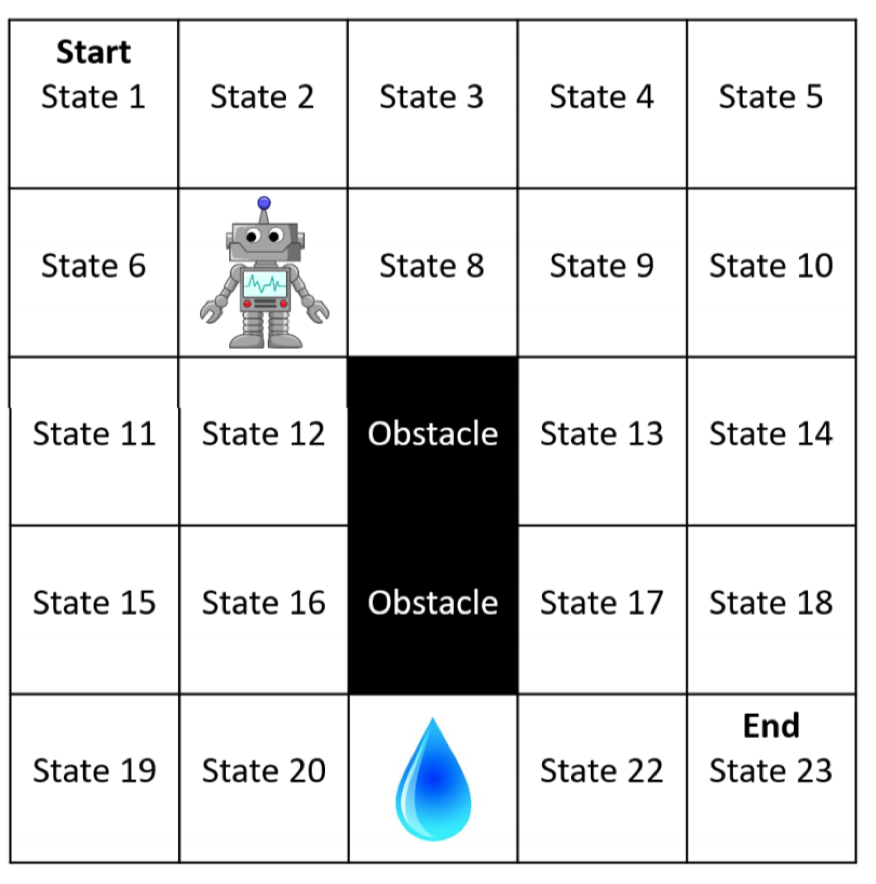
\includegraphics[width=0.3\textwidth]{HW_figs/687_gridworld.png}
    \caption{The original 687-GridWorld.}
    \label{fig:gridworld}
\end{figure}



\vspace{0.35in}
\noindent {\Large \textbf{2. Questions (Programming)}}

\vspace{0.15in}
General instructions:

\begin{itemize}
    \item You should initialize the value of all states to zero. 
    \item Whenever displaying values (e.g., the value of a state), use 4 decimal places; e.g, $v(s)=9.4312$.
    \item In the following questions, the Value Iteration algorithm should stop whenever $\Delta < 0.0001$.
    \item Unless otherwise specified, you should implement the ``standard'' version of Value Iteration: one that, at each iteration, performs a \textit{full backup}; and that is \textit{not} in-place (i.e., the updated value function, $v_{i+1}$, at iteration $i+1$, should be computed entirely based on $v_i$).
    \item Whenever showing the value function and policy learned by your algorithm, present them in a format resembling that depicted in Figure \ref{fig:output_format}.
\end{itemize}


\begin{figure}[!ht]
    \centering
    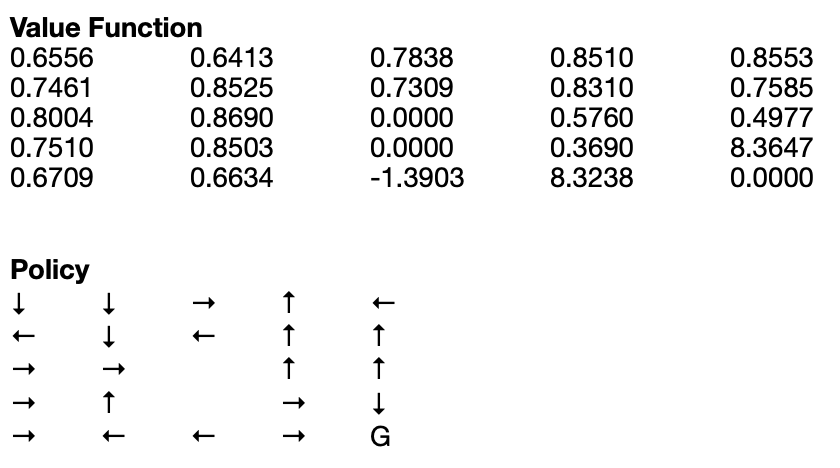
\includegraphics[width=0.45\textwidth]{HW_figs/output_format.png}
    \caption{Example of the output format your code should generate.}
    \label{fig:output_format}
\end{figure}


\begin{enumerate}
    \item (\POINTS{14 Points}) Run the Value Iteration algorithm in the 687-GridWorld as defined above until its stopping criterion is met. \textit{(a)} Show the final value function and the final policy identified by the algorithm. \textit{(b)} How many iterations did it take for the algorithm to stop? \textit{(c)} Describe, in English, the behavior being implemented by the learned  policy.
    %
    % YOUR RESPONSE HERE
    %
    
    
    \item (\POINTS{10 Points}) Run the same experiment as above, but now using $\gamma=0.25$. \textit{(a)} Show the final value function and the final policy identified by the algorithm. \textit{(b)} Did the value function identified when $\gamma=0.25$ change with respect to the value function identified when $\gamma=0.9$? How about the policy? If any of these quantities changed, explain, intuitively, why you think that happened. \textit{(c)} Finally, describe how many iterations it took for the algorithm to stop. Did it take more iterations or fewer iterations, compared to when $\gamma=0.9$? Explain, intuitively, why do you think that is the case.
    %
    %
    % YOUR RESPONSE HERE


    \item (\POINTS{10 Points}) In this question, you will once again use the Value Iteration algorithm with $\gamma=0.9$. You will now create a state in which the agent finds gold. To do so, change the reward given to the agent when entering the state $s=(0,2)$. Whenever that happens, the reward should be $5.0$. This should \textit{\ul{not}} be a terminal state. \textit{(a)} Show the final value function and the final policy identified by this algorithm. \textit{(b)} Describe, in English, the behavior being implemented by the learned policy, and explain intuitively why this is the best policy for this variant of the domain.
    %
    % YOUR RESPONSE HERE
    %
    
    
    \item (\POINTS{8 Points}) Repeat the experiment above but now make state $s=(0,2)$ a terminal state (similarly to the Goal state). Any actions executed in this state always transition to $s_\infty$ with reward $0$. \textit{(a)} Show the final value function and the final policy identified by the algorithm. \textit{(b)} Describe, in English, the behavior being implemented by the learned policy, and explain intuitively why this is the best policy for this variant of the domain. \textit{(c)} Finally, experiment with larger values of $\gamma$. What is the first larger value of $\gamma$ that causes the optimal policy to change---e.g., that causes the agent to avoid the new rewarding state? Describe intuitively why changing $\gamma$ in this way results in such a different behavior.
    %
    % YOUR RESPONSE HERE
    %
    
    
    \item (\POINTS{8 Points}) Repeat the experiment above (using $\gamma=0.9$) but now experiment with other rewards for entering $s=(0,2)$; i.e., rewards different than $5.0$. \textit{(a)} What is the first (smaller) reward value that causes the optimal policy to change---for instance, that causes the agent to avoid the new rewarding state? Describe intuitively why changing the reward in this way results in this new, different behavior. \textit{(b)} Show the final value function and the final policy identified by the algorithm.
    %
    % YOUR RESPONSE HERE
    %



\end{enumerate}


\end{document}